%%%%%%%%%%%%%%%%%%%%%%%%%%%%%%%%%%%%%%%%%%%%%%%%%%%%%%%%%%%%%%%%%%%%%%%%%%%%%%%%
%2345678901234567890123456789012345678901234567890123456789012345678901234567890
%        1         2         3         4         5         6         7         8

\documentclass{article}  % Comment this line out if you need a4paper
\usepackage{ijcai16}
\usepackage{times}
\usepackage{algorithmic}
\usepackage{algorithm}
\usepackage{subcaption}
%\documentclass[a4paper, 10pt, conference]{ieeeconf}      % Use this line for a4 paper

% See the \addtolength command later in the file to balance the column lengths
% on the last page of the document

% The following packages can be found on http:\\www.ctan.org
%\usepackage{graphics} % for pdf, bitmapped graphics files
%\usepackage{epsfig} % for postscript graphics files
%\usepackage{mathptmx} % assumes new font selection scheme installed
%\usepackage{times} % assumes new font selection scheme installed
%\usepackage{amsmath} % assumes amsmath package installed
%\usepackage{amssymb}  % assumes amsmath package installed

\title{\LARGE \bf
Rapidly Exploring Learning Trees
}
\usepackage{mathtools}
\usepackage{amsmath}
\usepackage{amsfonts}
\usepackage{color}
\usepackage{amssymb}
\DeclareMathOperator*{\argmin}{\arg\!\min} 
\DeclareMathOperator*{\argmax}{\arg\!\max} 
\author{Kyriacos Shiarlis \\
University of Amsterdam \\
k.c.shiarlis@uva.nl
\And 
Joao Messias \\
University of Amsterdam \\ 
jmessias@uva.nl 
\And
Shimon Whiteson \\
University of Oxford \\
shimon.whiteson@cs.ox.ac.uk 
}
\newcommand{\jm}[1]{\textcolor{blue}{Joao: #1}}

\newcommand{\sw}[1]{\textcolor{red}{SW: #1}}
\newcommand{\ks}[1]{\textcolor{green}{SW: #1}}


\begin{document}



\maketitle
\thispagestyle{empty}
\pagestyle{empty}


%%%%%%%%%%%%%%%%%%%%%%%%%%%%%%%%%%%%%%%%%%%%%%%%%%%%%%%%%%%%%%%%%%%%%%%%%%%%%%%%
\begin{abstract}
Inverse Reinforcement Learning (IRL) for path planning enables robots to learn cost functions for difficult tasks from demonstration, instead of hard-coding them. However, IRL methods face practical limitations that stem from their reliance on Markov decision process planners.
In this paper, we propose Rapidly Exploring Learning Trees (RLT$^*$), which learns the cost functions of Rapidly Exploring Random Trees (RRT) from demonstration, thereby making inverse learning methods applicable to more complex tasks. Our approach extends the Maximum Margin Planning to work with RRT$^*$ cost functions. Furthermore, we propose a caching scheme that greatly reduces the computational cost of this approach. Experimental results on real and simulated data from a social navigation scenario show that RLT$^*$ achieves better performance at lower computational cost than existing methods.

\end{abstract}


%%%%%%%%%%%%%%%%%%%%%%%%%%%%%%%%%%%%%%%%%%%%%%%%%%%%%%%%%%%%%%%%%%%%%%%%%%%%%%%%
\section{Introduction}

Learning from demonstration (LfD) \cite{argall2009survey} is of great interest to roboticists because it can avoid the need for tedious manual programming of complex behaviours. While most LfD methods rely on supervised learning to directly learn policies, certain approaches, namely inverse optimal control (IOC) \cite{kalman1964linear} and inverse reinforcement learning (IRL) \cite{abbeel2004apprenticeship} instead learn \emph{cost functions} from demonstration. These cost functions are then used to \emph{plan} the robot's behaviour. 

Cost functions tend to be more general and robust to changes in the environment such as friction in a manipulator's joints. A robot trained in a supervised manner has less chance of adapting than one that has been trained using IRL or IOC because the cost function remains unchanged. In addition, cost functions are thought to be more succinct representations of the aims of the agent \cite{abbeel2004apprenticeship}. %For example, an agent that whose aim is to get as fast as possible to a goal location. The policy for such an agent will be much harder to interpret when compared to its cost function. 

However, inverse methods also have practical limitations. IRL for example requires modeling the task as a Markov decision process (MDP), which is typically impractical in robotics, for several reasons.  Firstly, an MDP assumes full observability. Secondly, planning in an MDP, which IRL methods must do repeatedly, is costly, especially in continuous and high-dimensional domains. Finally, the lack of scalability and the assumption of full observability prohibit the natural modeling of important factors such as kinodynamic constraints. 

For these reasons, several researchers have proposed replacing the planning step in IRL with more convienient planners, e.g., Maximum Margin Planning (MMP) \cite{ratliff2006maximum} uses $A^*$ search for planning. This avoids the need to do all the planning in advance, as is typical when solving an MDP. It also avoids the need to model all aspects of the environment since the robot can quickly replan its trajectory to account for uncertainty. However, deterministic search methods such as A$^*$ require discretisation of the state space, and quickly run into scalability problems as the discretisation becomes finer. Furthermore, this discretisation again ignores kinodynamic constraints.

In path planning, Rapidly Exploring Random Trees (RRTs) \cite{lavalle1998rapidly} are popular because they cope well with continuous and high-dimensional domains and can elegantly handle kinodynamic constraints. The RRT$^*$ algorithm \cite{karaman2011sampling}, which extends RRTs to incorporate a cost function, is especially effective. However, the cost functions used by RRT$^*$ are typically simple and hand-coded and, to our knowledge, no methods have been developed to learn RRT$^*$ cost functions from demonstrations.

In this paper, we propose Rapidly Exploring Learning Trees (RLT$^*$), which learns RRT$^*$ cost functions from demonstration. Specifically we modify Maximum Margin Planning to use RRT$^*$ as a planner. Furthermore, we propose a caching scheme that greatly reduces the computational cost of this approach. RLT$^*$ requires no additional planner assumptions other than those inherent in RRT$^*$, making it particularly easy to implement. 

We evaluate RLT$^*$ on real and simulated data from a social navigation scenario. The results demonstrate that RLT$^*$ achieves better performance at lower computational cost than methods that learn path planning cost functions for deterministic planners.

\section{Related Work}

\sw{General IRL related work here.}

Substantial research has applied IRL to robotics \cite{henry2010learning,abbeel2008apprenticeship,vasquez2014inverse}. Because of the need to model the environment as an MDP, researchers usually discretise the state-action space. This introduces several key limitations. First, the size of the state-action space encountered in robotics is often prohibitive for such models. Second, the specific kinodynamic constraints of the robot cannot be easily be expressed by such representations, as they introduce non-Markovian dynamics. 

% \ks{Depending on the state-action space discretisation, past actions can infuence how easy it is to move to any a subsequent state. However the transition function only considers only one action in the past, and it is therefore an expectation over possible past configurations. As a result it tends to give the wrong probability distribution over next states for the actual physical system. Do I have to explain this in detail? Maybe Joao has a citation from his research?}

To apply IRL to more realistic situations, researchers usually try to replace the MDP model while retaining the main idea behind IRL, i.e., learning the underlying cost function of a planner using data from demonstrations. Maximum Entropy IRL \cite{ziebart2010modelingthesis} works in domains with linear continuous dynamics with the optimal controller being a Linear-Quadratic Regulator. Since linear dynamics are hard to come by in robotics, \cite{2012-cioc} considers locally linear aproximations. These bring about locally consistent rewards and achieve good performance in a range of tasks that were previously too hard for MDPs. However, the optimisation of the cost function using such planners is not guaranteed to be optimal. As our method is based on an RRT$^*$ planner, it is asymptotically optimal.

Other approaches to the problem use hybrid planners. Inverse Optimal Heuristic Control \cite{ratliff2009inverse} models the long-term goals of the agent as a coarse state MDP, to ensure tractability, while using supervised learning to determine the local policy of the agent at each state. Graph-Based IOC \cite{byravan2015graph} uses discrete optimal control on a coarse graph and the actual path is executed using local trajectory optimisation techniques such as CHOMP \cite{ratliff2009chomp}, which would otherwise suffer from local minima. The method is effective in robotic manipulation tasks with many degrees of freedom.  However, these methods employ complex and domain-specific planning formulations that are not suitable for all robotics tasks. The method presented here employs widely used planners, making it versatile and easy to implement. 

Another more recent graph-based concept is that of Adaptive State Graphs \cite{okallearning}, which build a controller graph before doing any learning. This controller graph is akin to \emph{options} in semi-Markov decision processes, and allows for a more flexible representation of the state-action space. However, the controller used to learn underlying cost function is not the same as the one used to execute the robot's behaviour. \sw{Why is that bad?}

RLT$^*$ can also be viewed as a graph-based, or rather tree-based, approach. Instead of building a controller graph first and then using different controllers to optimise trajectories, RLT$^*$ builds a controller tree on the fly.


\section{Background}
We begin with background on path planning and inverse reinforcement learning for path planning.

\subsection{Path Planning \label{subsec:path_planning}}
Path planning occurs in a space $\mathcal{S}$ of possible configurations of the robot. A configuration $s \in \mathcal{S}$ is usually continuous, and often represents spatial quantities such as position and orientation. A path planner seeks an obstacle-free path $\zeta_{o,g} = (s_1,s_2,s_3$ $\ldots,s_{l_{\zeta}}) $ of length $l_{\zeta}$, from an initial configuration $o = s_1$ to a goal configuration  $g =s_{l_{\zeta}}$. When the initial and goal configurations are implied, we refer to a path as $\zeta$.

Because there could be several paths to the goal, path planners typically employ a \emph{cost functional}, $C(\zeta)$ often defined as the sum of the costs between two subsequent configurations in a path $c(s_i,s_j)$. The total cost $C(\zeta)$ is therefore the sum of the individual costs along the path, i.e.,
\begin{equation}
	C(\zeta) = \sum_{i=0}^{l_{\zeta}-1} c(s_i,s_{i+1}).
\end{equation} \sw{Shouldn't it be $i=1$?}
This cost functional is similar to the one encountered in optimal control as well as to value functions used in reinforcement learning. Given the cost functional, the path planner seeks an optimal path $\zeta^*$, which satisfies,
\begin{equation}
 	\zeta^*_{o,g} = \argmin_{\zeta_{o,g} \in Z_{o,g}} C(\zeta), \label{eq:back_plan}
\end{equation}
where $Z_{o,g}$ is the set of all possible paths such that $s_1 = o, s_{l_\zeta} = g$.

Many path planning algorithms discretise $\mathcal{S}$ and use graph search algorithms like $A^*$ to find the optimal path. Under mild assumptions, these approaches are guaranteed to find the best path on the graph, but not in $\mathcal{S}$. However, they scale poorly in the size of $\mathcal{S}$, as larger and larger graphs are required. Furthermore, such methods do not address kinodynamic constraints, i.e., they assume that every configuration on the graph is accessible from a neighbouring one. 

These drawbacks motivate \emph{sample-based} path planning algorithms such as RRT$^*$. Instead of building a graph and then searching it, RRT$^*$ builds a tree on the fly and keeps track of the current best path. This tree can be grown in a way that respects kinodynamic constraints. Furthermore, a sampled-based approach can quickly find good, but not optimal, paths in large configuration spaces.

%  RRT$^*$ is also asymptotically optimal, i.e., it is guranteed to find an optimal path in $\mathcal{S}$ as the sampling time goes to infinity. Many variants of RRT$^*$ provide improved performance and faster convergence in practice by, for example, heuristically shriking the sampling space \cite{gammell2014informed}.

% The most significant difference between A$^*$ and RRT$^*$ is that while former is deterministic, the latter is probabilistic. It is important to understand how this distinction affects learning.

A$^*$ can solve \eqref{eq:back_plan} for a subset $\tilde{Z}_{o,g} \in  Z_{o,g}$ that is determined by its resolution (discretisation). RRT$^*$, for a given time budget T, also minimises a subset but in this case $\tilde{Z}_{o,g}$ is determined by the randomly sampled points. As $T \rightarrow \infty$, RRT$^*$ minimises over the entire $Z_{o,g}$, i.e., it is asymptotically optimal. In other words, the RRT$^*$ is asymptotically optimal as a function of sampling time and A$^*$ is asymptotically optimal as a function of resolution. %This distinction will become very important when we attempt to learn cost functions for these planners in the next section.

\subsection{IRL for Path Planning \label{subsec:inverse_problem}}
Path planning involves finding a (near) optimal path to the goal given a cost function. In the inverse problem, we are given example paths and must find the cost function for which these paths are (near) optimal.  The example paths comprise a dataset $\mathcal{D} = (\zeta^1_{o_1,g_1},\zeta^2_{o_2,g_2}...\zeta^D_{o_D,g_D})$ where $\zeta^i_{o_i,g_i}$ is an example path with initial and final configurations $o_i,g_i$ respectively. We assume the unknown cost function is of the form,
\begin{equation}
	c(s_i,s_j) = \mathbf{w}^T \mathbf{f}(s_i,s_j), \label{eq:inner_prod}
\end{equation}
where $\mathbf{f}(s_i,s_j)$ is a $K$-dimensional vector of features that encode different aspects of the configuration pair and $\mathbf{w}$ is a vector of unknown weights to be learned. Since $\mathbf{w}$ is independent of the configuration, we can express the total cost of the path in a parametric form:

\begin{equation}
	C(\zeta) = \mathbf{w}^T\sum_{i=0}^{l_{\zeta}-1} \mathbf{f}(s_i,s_{i+1}) := \mathbf{w}^T \mathbf{F}(\zeta),
\end{equation}
where $\mathbf{F}(\zeta)$ is the \emph{feature sum} of the path.

While many formulations of the inverse problem exist, the general idea is to find a weight vector that assigns less cost to the example paths than all other possible paths with the same initial and goal configuration.  This can be formalised by a set of inequality constraints:

\begin{equation}
	C(\zeta^i_{o_i,g_i}) \leq  C(\zeta) \quad \forall \zeta \in Z_{o_i,g_i}  \quad \forall i. \label{eq:const1}
\end{equation}
The constraint is an inequality because $Z_{o,g}$ contains only paths available to the planner and thus may not include the example path $\zeta^i_{o_i,g_i}$.
$Z_{o_i,g_i}$ can be large but if we have an optimisation procedure that solves \eqref{eq:back_plan}, it is enough to satisfy, 
\begin{equation}
	C(\zeta^i_{o_i,g_i}) \leq \min_{\zeta \in Z_{o_i,g_i}} C(\zeta) \quad \forall i, \label{eq:const}
\end{equation}

Ratliff et al.\ \cite{ratliff2006maximum} propose a maximum margin variant of \eqref{eq:const} by introducing a margin function $L_i(\zeta)$ that decreases the cost of the proposed path $\zeta$ if is dissimilar to $\zeta^i_{o_i,g_i}$. For example, $L_i(\zeta)$ could be $-1$ times the number of configurations in the demonstration path not visited by $\zeta$. The full optimisation formulation of Maximum Margin Planning is as follows.

\begin{equation}
	\argmin_{\mathbf{w},\tau} \frac{1}{2}||\mathbf{w}||^2 + \frac{\lambda}{D} \sum_i \tau_i \label{eq:mas_marg}
\end{equation}
\begin{equation}
	\text{s.t.} \quad C(\zeta^i_{o_i,g_i}) - \tau_i \leq \min_{\zeta \in Z_{o_i,g_i}} C(\zeta) + L_i(\zeta) \quad \forall i,
\end{equation}
where $\tau_i$ are slacks that can be used to relax the constraints. Rearranging the inequality in terms of the slacks we get:

\begin{equation}
	 \quad C(\zeta^i_{o_i,g_i}) - \min_{\zeta \in Z_{o_i,g_i}} C(\zeta) + L_i(\zeta)  \leq \tau_i  \quad \forall i.
\end{equation}
Consequently, the $\mathbf{w}$ minimising:
\begin{equation}
	\frac{1}{2}||\mathbf{w}||^2 + \frac{\lambda}{D} \sum_i \big( C(\zeta^i_{o_i,g_i}) - \min_{\zeta \in Z_{o_i,g_i}}\big(C(\zeta) + L_i(\zeta)\big) \big) \big. \label{eq:unconstrained}
\end{equation}
is equivalent \eqref{eq:mas_marg}, i.e., the slacks are tight.
The minimum can be found by computing a subgradient and performing gradient descent on the above objective:
\begin{equation}
	\nabla_{\mathbf{w}} =\mathbf{w} +  \frac{\lambda}{D} \sum_{i=0}^D F(\zeta^i_{o_i,g_i}) - F(\tilde{\zeta}^*_{o_i,g_i}), \label{eq:update1}
\end{equation}
where,
\begin{equation}
	\tilde{\zeta}^*_{o_i,g_i} = \argmin_{\zeta \in Z_{o_i,g_i}} C(\zeta) + L_i(\zeta). \label{eq:augmented_max}
\end{equation}

The inverse problem can therefore be seen as an iterative procedure, that first solves \eqref{eq:augmented_max} in the inner loop while keeping the weights constant. Based on that solution, it updates the weights using \eqref{eq:update1} in the outer loop. The weights at convergence represent the cost function that is used to plan the future behaviour of the agent. In \cite{ratliff2006maximum}, A$^*$ search was used for planning in the inner loop, assuming that the domain contained acyclic positive costs. In this paper, we make the same assumptions but develop methods that use RRT$^*$ for planning.

\section{Method}
	In this section, we propose Rapidly Exploring Learning Trees (RLT$^*$).  We first propose a generic extension to the maximum margin approach that we call Approximate Maximum Margin Planning.  We then show how an implementation of this approach with an RRT$^*$ planner and a novel caching scheme yields RLT$^*$.

	% \subsection{Feature Sums and Sampled Based Planners}
	% 	Feature sums, $F(\zeta)$, can be seen as the  `fingerprints' of paths, and their definition is of crucial importance in the inverse problem. When planning on a fixed graph, like in the case of MDPs or A$^*$ search, it is easy to define the feature sums as the \emph{edge} costs on the graph. Furthermore if planning in continous domains we may consider integrals along the path. In RRT's however the tree that is being built has neither a fixed structure, nor an analytical form. Thus, the first step towards learning RRT$^*$ cost functions from demonstration is to come up with a reasonable approximation of $F(\zeta)$ for a path. This approximation must be consistent with the definition of the cost for a configuration pair. One such definition for cost is as follows.
	% 	\begin{equation}
	% 		c(s_i,s_j) = \frac{c(s_i)+c(s_j)}{2}d_{s_i,s_j}
	% 	\end{equation}
	% 	Where $c(s_i)$ is a cost function defined over a single configuration and $d_{s_i,s_j}$ is a measure of distance between the two configurations. For example if we consider configurations to be points in Eucledian space then $d_{s_i,s_j}$ can be the eucledian distance. Noting that the costs and features are related by \eqref{eq:inner_prod} for a single feature $f_k$ we have,

	% 	\begin{equation}
	% 		f_k(s_i,s_j) = \frac{f(s_i)+f(s_j)}{2}d_{s_i,s_j}
	% 	\end{equation}
	% 	Following this definition feature sum calculation along a candidate path is trivial,
	% 	\begin{equation}
	% 		F(\zeta) = \sum_{i=0}^{\zeta_l-1} \frac{\mathbf{f}(s_i)+\mathbf{f}(s_{i+1})}{2}d_{s_i,s_{i+1}}
	% 	\end{equation}

	\subsection{Approximate Maximum Margin Planning \label{subsec:ammp}}

		In Section \ref{subsec:inverse_problem}, we showed how the multiple constraints of \eqref{eq:const1} could be reduced to a single constraint for each demonstration in \eqref{eq:const}. However, given a finite time budget $T$, a sample-based planner like RRT$^*$ minimises, not over the full set of paths $Z_{o,g}$, but over a randomly sampled $\tilde{Z}_{o,g}$. Thus, we can modify \eqref{eq:const}, and demand that our cost function satisfies,
\begin{equation}
	C(\zeta^i_{o_i,g_i}) \leq \min_{\zeta_{o_i,g_i} \in \tilde{Z}_{o_i,g_i}} C(\zeta) \quad \forall i. \label{eq:const_rrt}
\end{equation}
	As the planning budget T increases, the sample-based planner samples lower cost paths, making this inequality harder to satisfy. Assuming $\tilde{Z}_{o_i,g_i}$ is constant, we can rewrite \eqref{eq:unconstrained} as:

	\begin{equation} \frac{1}{2}||\mathbf{w}||^2 + \frac{\lambda}{D} \sum_i \big( C(\zeta^i_{o_i,g_i}) - \min_{\zeta \in \tilde{Z}_{o_i,g_i}}\big(C(\zeta) + L_i(\zeta)\big) \big). \label{eq:unconstrained_rrt}
	\end{equation}
	This gives rise to an approach we call Approximate Maximum Margin Planning (AMMP), which is similar  to the one described in Section \ref{subsec:inverse_problem}, with the crucial difference that the planning step is executed by a sample-based planner and not a deterministic one, like A$^*$. An important consequence is that $\tilde{Z}_{o_i,g_i}$ now changes every time we invoke the sample-based planner. As a result, AMMP can be thought of as a smart way of sampling the \emph{constraints} that we want our cost function to satisfy. 

\subsection{Rapidly Exploring Learning Trees \label{subsec:cached}}

A simple way to construct a concrete algorithm from AMMP is to use RRT$^*$ as the sample-based planner.  However, this results in a computationally expensive algorithm, which calls the planner $I\times|D|$ times over $I$ iterations given a dataset of size $|D|$.  Since planning is typically expensive, it is crucial to find a more efficient approach.

In this section, we propose Rapidly Exploring Learning Trees (RLT$^*$), which implements AMMP with an RRT$^*$ planner but uses a caching scheme to achieve computational efficiency.

Two of the most costly operations of RRT$^*$ are 1) finding the nearest neighbour to a newly sampled point and 2) finding the radius-neighbours of a newly created vertex in the tree \cite{karaman2011sampling}. However, a key observation is that neither of these procedures depend on the cost function used by the planner. Thus,  RRT$^*$ can be split in two independent steps. 

	The first step is described in Algorithm \ref{alg:rrt_cache}, which takes as input $p$, the number of points to randomly sample from free space; $s_{init}$, the initial point; and $\eta$, the steer step size. For each randomly sampled point $s_{rand}$, we find the nearest neighbour, $s_{nearest}$, from the set of points in the vertex set $V$. We then create a new configuration point $s_{new}$ by steering from $s_{nearest}$ to $s_{rand}$. Next, we query the radius neighbours of $s_{new}$ at a radius determined by  $\min\{\gamma_{RRT^*}(\frac{\log(|V|)}{|V|})^{\frac{1}{d}},\eta\}$. Here, $d$ is the dimensionality of $S$, and $\gamma_{RRT^*}$ is a constant based on the volume of free space (see \cite{karaman2011sampling}). The points $s_{new}$, $s_{nearest}$ and the set $S_{near}$ are stored together in the map $P$, which we call the \emph{point cache}, and is returned at the end of the procedure. This algorithm turns the sampling process of RRT$^*$  into a preprocessing step. Consequently, the expensive \texttt{Nearest} and \texttt{Near} procedures only need to be repeated $|D|$ times instead of $I\times|D|$ times.


	\begin{algorithm}
	\caption{\texttt{cacheRRT}($p$,$s_{init}$,$\eta$)}
	\label{alg:rrt_cache}
	\begin{algorithmic}[1]
	\STATE $P \gets \emptyset$ \hfill \COMMENT{Initialise the point cache}
	\STATE $V \gets {s_{init}}$
	\FOR{$i=0 \dots p $}
	\STATE $s_{rand} \gets SampleFree_i$
	\STATE $s_{nearest} \gets \texttt{Nearest}(V,s_{rand})$
	\STATE $s_{new} \gets \texttt{Steer}(s_{nearest},s_{rand})$
	\STATE $S_{near} \gets \texttt{Near}(V,{s_{new}},\min\{\gamma_{RRT^*}(\frac{\log(|V|)}{|V|})^{\frac{1}{d}},\eta\})$ 
	\STATE $V\gets V \cup s_{new}$
	\STATE $P \gets P \cup \{s_{new},S_{near}\}$
	\ENDFOR
	\RETURN $P$

	\end{algorithmic}
	\end{algorithm}

The output of Algorithm \ref{alg:rrt_cache} is input to Algorithm \ref{alg:plan_cached}, which resembles wiring and re-wiring procedures in RRT$^*$ \cite{karaman2011sampling}, and returns a minimum cost path to the goal. An important difference, however, is that the vertices of the tree and their neighbours at each iteration are already known and contained within the point cache. This speeds computation while keeping consistency between the planners used during learning and final execution. As learning proceeds and the cost function changes, so does the wiring of this tree; however, the points involved do not change.

	\begin{algorithm}
	\caption{\texttt{planCachedRRT$^*$}($P$,$s_{init}$,$c()$)}
	 \label{alg:plan_cached}
	\begin{algorithmic}[1]
	\STATE $E \gets \emptyset$
	\STATE $V \gets {s_{init}}$
	\FOR{$i=0 \dots |P| $}
	\STATE $s_{nearest} \gets P\{s_{nearest}^i\}$
	\STATE $s_{new} \gets P\{s_{new}^i\}$
	\STATE $S_{near} \gets P\{S_{near}^i\}$
	\STATE $V\gets V \cup s_{new}$
	\STATE $s_{min}\gets s_{nearest}$
	\STATE $c_{min}\gets \texttt{Cost}(s_{nearest}) + c(s_{nearest},s_{new})$
	\FOR{$s_{near} \in S_{near} $}
	\STATE $c_{near} \gets \texttt{Cost}(s_{near}) + c(s_{near},s_{new})$
	\IF {\texttt{CollisionFree}($s_{near},s_{new}$) and  $c_{near}<c_{new}$}
	\STATE $s_{min} \gets s_{near}; c_{min}\gets c_{near}$
	\ENDIF
	\ENDFOR
	\STATE $E \gets E \cup \{(s_{min},s_{new})\} $
	\FOR{$s_{near} \in S_{near} $}
	\STATE $c_{new} \gets \texttt{Cost}(s_{near}) + c(s_{near},s_{new})$
	\IF {\texttt{CollisionFree}($s_{near},s_{new}$) and  $c_{new}<\texttt{Cost}(s_{near})$}
	\STATE $s_{parent} \gets \texttt{Parent}(s_{near})$
	\STATE $E \gets E  \smallsetminus {(s_{parent},s_{near})} \cup {(s_{new},s_{near})} $
	\ENDIF
	\ENDFOR
	\ENDFOR
	\STATE $\zeta_{min} \gets \texttt{minCostPath}(V,E,c())$
	\RETURN $\zeta_{min}$

	\end{algorithmic}
	\end{algorithm}

Algorithm \ref{alg:ammp} describes Rapidly Exploring Learning Trees (RLT$^*$), which uses  Algorithms \ref{alg:rrt_cache} and \ref{alg:plan_cached}. First, we initialise the weights, either randomly or using a cost function that simply favours shortest paths. Then, for each datapoint $\zeta_i$, we calculate feature sums and run \texttt{cacheRRT}. The main learning loop involves cycling through all data points and finding the best path under a loss-augmented cost function. The feature sums of this path are calculated and subsequently the difference with the demonstrated feature sums is computed. At the end of each iteration, an average gradient is calculated and the cost function is updated. At convergence, the learned weights are returned.

	\begin{algorithm}
	\caption{\texttt{RLT$^*$}($D,p,\eta,\lambda,\delta$)\label{alg:ammp}}
	\begin{algorithmic}[1]
	\STATE $\mathbf{w} \gets \texttt{initialiseWeights}$
	\STATE $\mathbf{\tilde{F}} \gets \emptyset$
	\STATE $R \gets \emptyset$
	\FOR{$\zeta^i \text{ in } D$}
	\STATE $\tilde{F}_{\zeta^i} \gets \texttt{FeatureSums}(\zeta^i)$
	\STATE $\mathbf{\tilde{F}} \gets \mathbf{\tilde{F}} \cup \tilde{F}_{\zeta^i}$
	\STATE $r_i \gets \texttt{cacheRRT}(p,s_{init}^{\zeta^i},\eta)$
	\STATE $R \gets R \cup r_i $
	\ENDFOR
	\REPEAT
	\STATE $\nabla_{\mathbf{w}}\gets 0$
	\FOR{$ \zeta^i \text{in } D $}
	\STATE $c() \gets \texttt{getCostmap}(\mathbf{w}) + L(\zeta^i)$ 
	\STATE $r_i \gets R\{i\}$ ;	$\tilde{F}_i \gets \mathbf{\tilde{F}}\{i\}$ 
	\STATE $\zeta \gets \texttt{planCachedRRT}^*(r_i,x^i_{init},c())$
	\STATE $F_i \gets \texttt{FeatureSums}(\zeta)$
	\STATE $\nabla_{\mathbf{w}} \gets \nabla_{\mathbf{w}} + \tilde{F}_i - F_i $
	\ENDFOR
	\STATE $\nabla_{\mathbf{w}} \gets \mathbf{w} + \frac{\lambda}{|D|}\nabla_{\mathbf{w}} $
	\STATE $\mathbf{w} \gets \mathbf{w} - \delta\nabla_{\mathbf{w}} $
	\UNTIL{convergence}
	\RETURN $V,E$

	\end{algorithmic}
	\end{algorithm}

	% \STATE $\widetilde{\mu}^{\mathcal{D}} \gets \mathtt{empiricalFE}(\mathcal{D})$\hfill \COMMENT{using \eqref{eqn:empirical_fe}}
	% \STATE $\widetilde{\mu}^{\mathcal{F}} \gets \mathtt{empiricalFE}(\mathcal{F})$ 
	% \STATE $P_{\mathcal{D}}^{s_1} \gets \mathtt{initialStateDistribution}(\mathcal{D})$
	% \STATE $P_{\mathcal{F}}^{s_1} \gets \mathtt{initialStateDistribution}(\mathcal{F})$
	% \STATE $w^{\mathcal{F}}_k\gets 0\quad\forall k\in\{1,\ldots,K\}$
	% \REPEAT
	% \STATE $R(s,a) \gets (w^{\mathcal{D}}+w^{\mathcal{F}})^T\phi(s,a)\quad\forall s\in\mathcal{S},a\in\mathcal{A}$
	% \STATE $\pi \gets \mathtt{softPlan}(\mathcal{S},\mathcal{A},T,R)$\hfill\COMMENT{using \eqref{eq:soft_backup}}
	% \STATE $\mu^\pi|_{\mathcal{D}} = \mathtt{calculateFE}(\pi,T,P_{\mathcal{D}}^{s_1})$
	% \STATE $\mu^\pi|_{\mathcal{F}} = \mathtt{calculateFE}(\pi,T,P_{\mathcal{F}}^{s_1})$
	% \STATE $w^{\mathcal{D}} \leftarrow w^{\mathcal{D}} - \alpha (\mu^\pi|_{\mathcal{D}} - \widetilde{\mu}^{\mathcal{D}})$
	% \STATE $w^{\mathcal{F}} \leftarrow \frac{(\mu^\pi|_{\mathcal{F}} - \widetilde{\mu}^{\mathcal{F}})}{\lambda}$

	% \IF {$\lambda > \lambda_{min}$}
	% \STATE $\lambda \leftarrow \alpha_{\lambda}\lambda$
	% \ENDIF
	% \UNTIL{convergence}
	% \RETURN $R,\pi$


For RRT$^*$ the dependance of $\tilde{Z}_{o_i,g_i}$ on the time budget T is very hard to quantify since it also depends on the size and nature of $S$ as well as the cost function we are using -which also changes with every iteration. For this reason, in this paper we resort to an experimental assesment of the ability of RRT$^*$ to sample the right constraints at every iteration of RLT$^*$ and hence allow the learning of a cost function from a set of demonstrated paths.


\section{Experiments}
In this section, we experimentally compare RLT$^*$ to the original MMP algorithm implemented using an A$^*$ planner, as well as to an ablated version of RLT$^*$ that does not using caching.
	
	Our experiments take place in the context of socially intelligent navigation. IRL has been widely used in this setting \cite{okallearning,henry2010learning,vasquez2014inverse} because it is usually infeasible to hard-code the cost functions that a planner should use in complex social situations. Having the ability to quickly and effectively learn social navigation cost functions from demonstration would be a major asset for robots that operate in crowded environments such as airports \cite{triebel2015spencer}, museums \cite{thrun1999minerva} and care centres \cite{shiarlis2015teresa}.
	
	\subsection{Setting}
	Our experiments take place in a randomly generated social environment, shown in Figure \ref{fig:exp_setting}. Every arrow in the figure represents a person's position and orientation. The robot is given the task of navigating from one point in the room to another. While it is aware of the orientation and position of different people, it has no idea on how to trade off reaching the target quickly with avoiding people and obstacles, i.e., the cost function is unknown. Instead, the robot is given a dataset of demonstrations $D$. Each demonstration $\zeta_i$ is a set of configurations $s = (x,y)$ representing positions of the robot in the configuration space and each demonstration takes place for a different random configuration of the social environment, i.e., the people are at different positions and orientations every time. The task of the robot is to, using $D$, extract a cost function based on different features of the environment, which in turn would allow it to behave socially in future tasks.

	The features involved in our experiments include three Gaussian functions of different means and diagonal covariances around each person, three different functions that measure distance from the goal and a feature that measures proximity to obstacles. Figure \ref{fig:cost_f} shows an example cost function over the whole configuration space for the configuration in Figure \ref{fig:exp_setting}.


	\begin{figure}[tbh]
%	\hspace{-5cm}
      \begin{subfigure}[b]{0.435\columnwidth}

    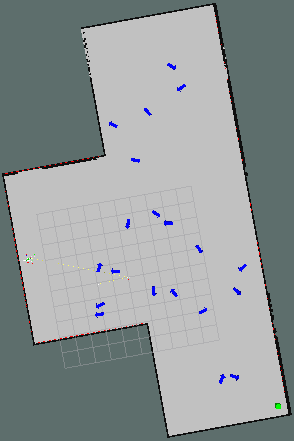
\includegraphics[width=0.9\textwidth]{images/people.png}
    \caption{Example setting }
    \label{fig:exp_setting}
  \end{subfigure}
  \hspace{10mm}
  \begin{subfigure}[b]{0.435\columnwidth}
    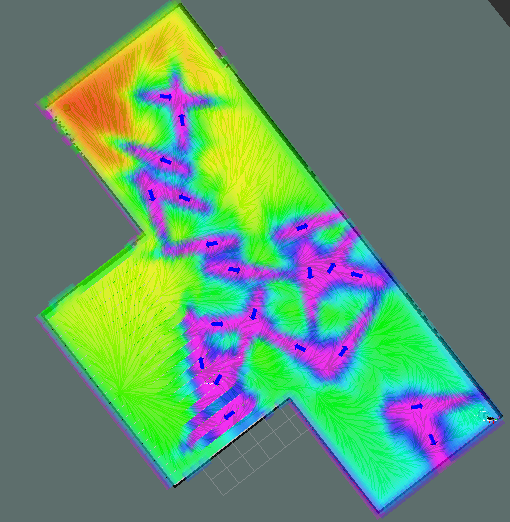
\includegraphics[width=0.9\textwidth]{images/cost_f.png}
    \caption{Cost function}
    \label{fig:cost_f}
  \end{subfigure} 

  %\vspace{-3mm}
  \caption{(a) An instance of the randomised social navigation task. Arrows denote the position and orientation of people in the scene. The robot is on the lefthand side of the map and the green box in the bottom right denotes the goal location. (b) The corresponding cost function for the random scenario. Red denotes \emph{low} cost, while purple denotes \emph{high} cost.}
  %\vspace{-3mm}
  \label{fig:setting}
  \end{figure}


	\subsection{Evaluation}

	To evaluate the effectiveness of our algorithms we employ both quantitative as well as qualitative comparisons.

	To quantitatively assess the quality of our algorithms, we generate a dataset $D$ by planning near-optimal paths from an initial configuration $s_o$ to a goal configuration $s_g$ under a ground-truth cost function $c_{gt}()$ derived from respective ground-truth weights $\mathbf{w}_{gt}$. A fully optimal path can only be derived only asymptotically in terms of either time  for RRT$^*$, or resolution for A$^*$. In practice, however, we found that planning for 60 seconds using  RRT$^*$  achieves a path that is nearly optimal, as running longer leads to negligible changes in path cost. 
	
	The resulting ground truth dataset is extremely useful for evaluation. For each path $\zeta$ generated by the learner, we know its cost under the ground-truth cost function is simply  $\mathbf{w}_{gt}\mathbf{F}(\zeta)$. Furthermore, we can compute the cost difference between the generated path and the example path:
	\begin{equation}
		Q(\zeta,\zeta_i,\mathbf{w}) = \mathbf{w}(\mathbf{F}(\zeta)-\mathbf{F}(\zeta_i)), \label{eq:obj_eval}
	\end{equation}
which is our primary performance metric.  Note that, if the demonstration path $\zeta_i$ is optimal under $\mathbf{w}$, then $Q(\zeta,\zeta_i,\mathbf{w})>=0$.

For our experiments, the ground-truth weights $\mathbf{w}_{gt}$ were chosen mainly induce a cost function that penalises passing in front of people. In addition, small weights were added to the other two Gaussian functions for each each individual person, as well as both linear and exponential penalisation of the distance from the goal, so that the resulting cost function, shown in Figure \ref{fig:cost_f}, would not be too trivial. 

We also measure the time per iteration of each learning algorithm.  All algorithms were implemented in Python, share similar functions, and were not optimised for speed apart from the caching scheme in RLT$^*$.

	We also perform qualitative evaluation of the algorithms by visually comparing the learned cost functions for each algorithm and the paths they generate against the ground truth cost function and the demonstration paths.

	\subsection{Results}

	Our dataset $D$ consists of 20 trajectories at random social situations within the social environment shown in Figure \ref{fig:exp_setting}, using the cost function shown in Figure \ref{fig:cost_f}. Half of these trajectories make up the training dataset $D_{train}$ and the other half the test dataset $D_{test}$. After being trained on $D_{train}$, the performance of a cost function is evaluated on $D_{test}$ using \eqref{eq:obj_eval}. The process is repeated four times for the same dataset but with different random compositions of $D_{train}$ and $D_{test}$. We report both the mean and standard error across the different trajectories in the test and training sets, for each iteration in Figures \ref{fig:train_results} and \ref{fig:test_results}. 

We report results for RLT$^*$, RLT$^*$ without caching, and MMP with A$^*$ at grid resolutions of 0.8 and 0.3 metres.  For RLT$^*$, we set the number of sampled points $p=2500$. For RLT$^*$ without 
caching, we cap planning at 12$s$, which is about how long RRT$^*$ plans for when $p=2500$.  Note 
that this is much less planning time than the 60$s$ used to generate the demonstrations.
 All learning algorithms were initialised using a cost function that only favours shortest paths.

The results show that both versions of RLT$^*$ always outperform both versions of MMP with A$^*$. This can be attributed to the fact that the underlying RRT$^*$ planner is not confined to work on a fixed grid, allowing it to generate paths that are closer to optimal. This is further reinforced by the increased performance as the grid resolution decreases allowing MMP$_{0.3}$ to approach the performance of RLT$^*$. Standard error rates are similar across methods.

	Table \ref{tab:time} shows the average planning time per learning iteration and the total learning time for all algorithms, along with their average cost difference on the test set at convergence. Comparing RLT$^*$ with and without caching shows that the cached version is much faster without a significant cost in performance. Furthermore both algorithms, although slower than MMP$_{0.8}$, are faster than MMP$_{0.3}$. This means that, even if a higher resolution MMP  was able to match the performance of RLT$^*$, it would be much slower. Furthermore, there is large variance in planning time for MMP$_{0.3}$. At the start of learning, the initial cost function is very simple and and only involves the distance from the goal location. Under this cost function, planning is quick, because a simple heuristic that simply takes into account the distance from the goal is a  good approximation to the cost-to-go. As learning proceeds, however, the cost function becomes more complex, and this simple heuristic, although admissible, is no longer tight. This requires the A$^*$ planner to expand many more states before an optimal path is found. We can see therefore that MMP with A$^*$ scales poorly, not only the size of $S$, but also in the complexity of the cost function. By contrast, the probabilistic nature of RLT$^*$ makes it less susceptible to these pathologies.  

	For a qualitative comparison, we look to Figures \ref{fig:path_compare} and \ref{fig:cfs}. Figure \ref{fig:path_compare} shows a demonstrated path (black) along with the paths generated by three of the four algorithms. Note the effect of planning on a coarse grid in the case of MMP$_{0.8}$ (green). We can also see that RLT$^*$ (red) more faithfully replicates the example path. Figure \ref{fig:cfs} compares the ground truth cost function (Figure \ref{fig:get_cf}) against the learned cost functions for  MMP$_{0.3}$ and RLT$^*$ (Figures \ref{fig:astar03_cf}, \ref{fig:rrt_cf}). This comparison shows that  MMP$_{0.3}$ overestimates the cost related with the distance from the goal, i.e., the cost increases faster as we move away from the goal. This yields paths that reach the goal earlier, possibly accounting for the small difference in performance between the two algorithms. 

\begin{figure}[tbh]
	\centering
%	\hspace{-5cm}
      \hspace{-5mm}
      \begin{subfigure}[b]{0.455\columnwidth}

    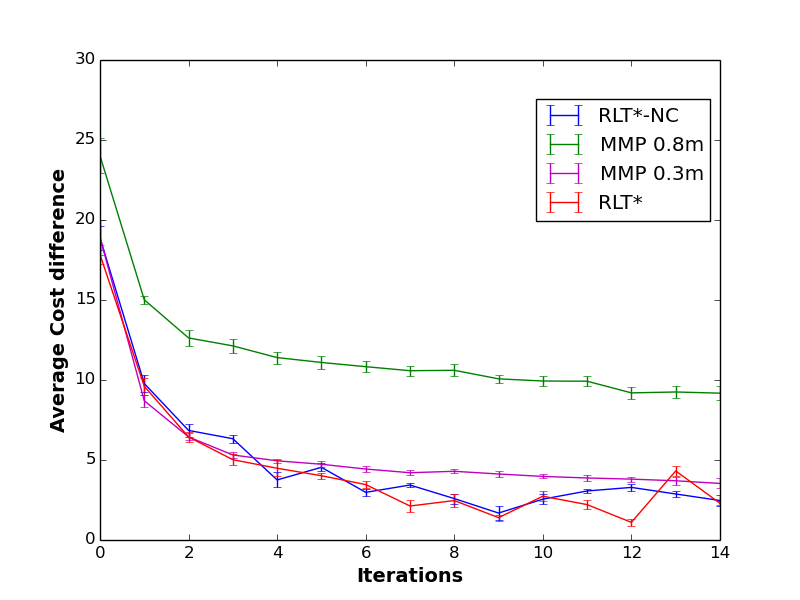
\includegraphics[clip=true,width=1.25\textwidth]{images/cost_diff_train.png}
    \caption{Train}
    \label{fig:train_results}
  \end{subfigure}
 % \hspace{5mm}
 \hspace{5mm}
  \begin{subfigure}[b]{0.455\columnwidth}
    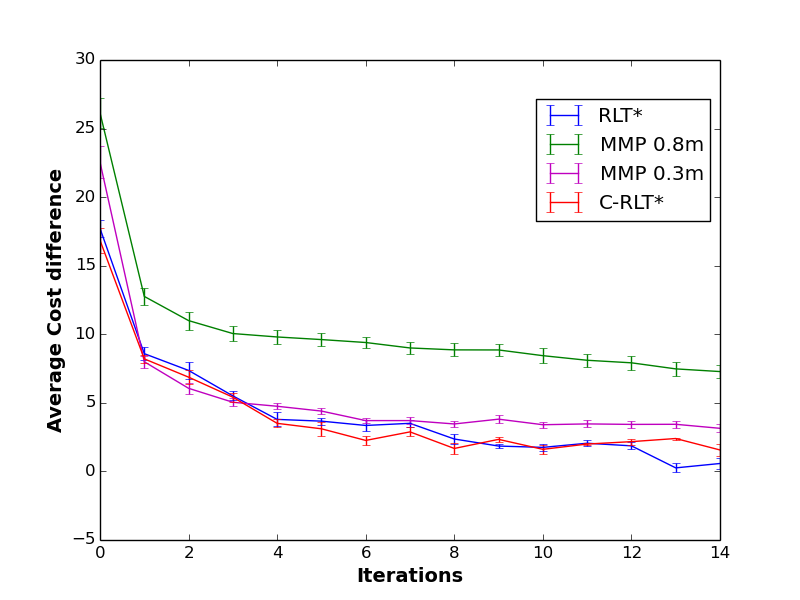
\includegraphics[clip=true,width=1.25\textwidth]{images/cost_diff_val.png}
    \caption{Test}
    \label{fig:test_results}
  \end{subfigure} 

  %\vspace{-3mm}
  \caption{Train and test set average cost difference, for 15 iterations. Error bars represent standard error over four independent runs on shuffled versions of the data. \sw{Update legend with new method names.}}
  %\vspace{-3mm}
  \label{fig:results}
\end{figure}

	\begin{table}[]
	\centering

	\begin{tabular}{|l|l|l|l|l|}
	\hline
	               & MMP$_{0.8}$     & MMP$_{0.3}$       & RLT$^*$-NC  & RLT$^*$ \\ \hline
	Iteration (s) & 1.83(0.79) & 20.93(12.14) & 12(0) & 5.87(0.50)  \\ \hline
	Learning (s) & 275.2      & 3140.6       & 1808  & 911.7       \\ \hline
	$Q(\zeta,\zeta_i,\mathbf{w}_{gt})$ & 7.28      & 3.14       & 0.57  & 1.57       \\ \hline
	\end{tabular}
	\caption{Per iteration and total learning times for our proposed algorithms and the baselines (RLT$^*$-NC is RLT$^*$ without caching. \sw{You need to make this table fit in a column width.}}
	\label{tab:time}
	\end{table}


	\begin{figure}
	\centering
	%\vspace{-3.3mm}
	    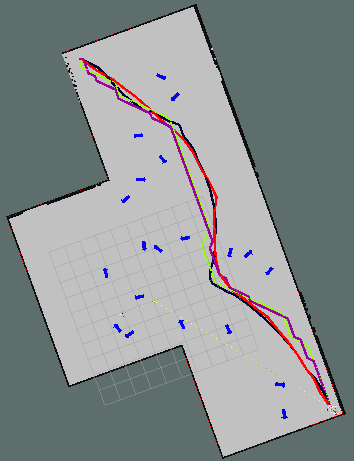
\includegraphics[width=0.20\textwidth]{images/path_compare.png}
	%\vspace{-4mm}
	  \caption{Qualitative comparison of paths. Goal is at the top left, robot begins on the bottom right. Black: demonstration path. Red: RLT$^*$. Green: MMP$_{0.8}$, Magenta: MMP$_{0.3}$ }
	  \label{fig:path_compare}
	\end{figure}


	\begin{figure}[tbh]
	\hspace{5mm}
      \begin{subfigure}[b]{0.3\columnwidth}
    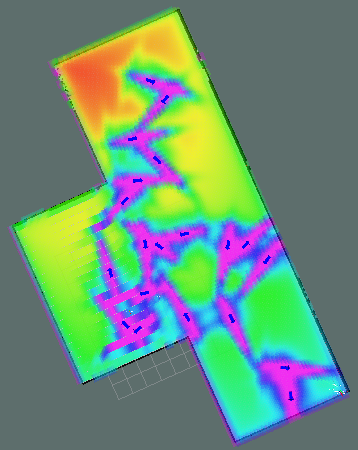
\includegraphics[width=1.\textwidth]{images/gt_ct.png}
    \caption{Ground truth}
    \label{fig:get_cf}
  \end{subfigure}
  %\hspace{1mm}
  \begin{subfigure}[b]{0.292\columnwidth}
    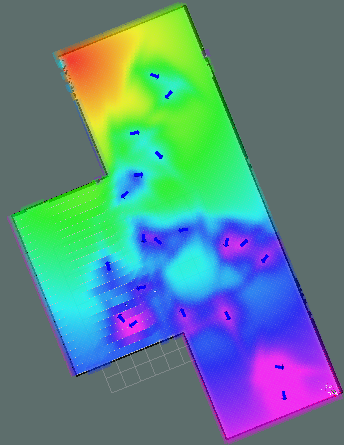
\includegraphics[width=1.\textwidth]{images/astar03.png}
    \caption{MMP$_{0.3}$}
    \label{fig:astar03_cf}
   \end{subfigure}
   %\hspace{1mm}
  \begin{subfigure}[b]{0.296\columnwidth}
    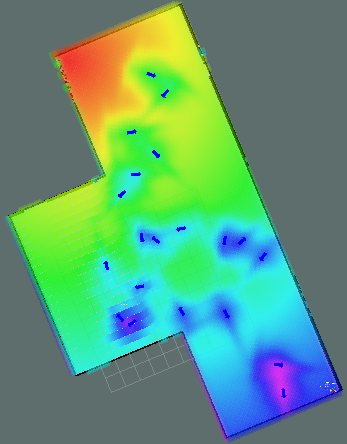
\includegraphics[width=1.\textwidth]{images/rrt_cf.png}
    \caption{C-RLT$^*$}
    \label{fig:rrt_cf}
  \end{subfigure} 
  	  \caption{Ground truth and learned cost functions using MMP$_{0.3}$ and RRT$^*$.  \label{fig:cfs}}
  \end{figure}


\section{Conclusion and Future Work}
In this paper, we proposed Rapidly Exploring Learning Trees (RLT$^*$), which learns the cost functions of Rapidly Exploring Random Trees (RRT) from demonstration, thereby making inverse learning methods applicable to more complex tasks. Our approach extends the Maximum Margin Planning to work with RRT$^*$ cost functions. Furthermore, we proposed a caching scheme that greatly reduces the computational cost of this approach. Experimental results on real and simulated data from a social navigation scenario showed that RLT$^*$ achieves better performance at lower computational cost than existing methods.

 Although our experimental comparison used A$^*$ as a baseline, RLT$^*$ is also well suited to situations where deterministic planners naturally fail, e.g., a manipulator with many degrees of freedom. A clear avenue for future work is to design learning algorithms that explicitly take into account the probabilistic nature of RRT$^*$. We also plan to evaluate RLT$^*$ on data gathered from real robots.

\bibliographystyle{IEEEtran}
\bibliography{references}



\end{document}
